\section{Memoryless Deterministic Reflex Agent}
For this task, we are trying to design the simplest agent with limited number of if-then rules. Since there are 3 sensors for wall, dirty and home grid, the agent may face $2^3$ different cases. The idea behind the memoryless agent is based on the (situation, action) pairs. For simplicity, we assume that the agent will only take one step for each situation, and then he forget what he has done. The designed rules are inserted into the main loop to control his actions. So the task here is to learn a mapping $f(wall, dirty, home)$ for the action space.   

\subsection{Is It Able To Finish}
Before coding these rules, we are thinking about a question that: is it possible to finish the cleaning task only with the one-to-one mapping? For answering this question, we make a simple experiment on each type of cell to see if an agent can travel through it. We show a $4 \times 4$ map in figure \ref{fig:celltypes}, in which we can see in fact there are three types of cells. The diamond cells (corner cells) or circle cells (border cells) can be easily to access, just let the agent go ahead when
there is no wall and turn left or right when facing a wall. But how about the triangle cells? Can it step into such a cell? If so, we can make sure that the memoryless can finish the task properly. Let's look at the triangle cell. There are only four ways to step into the central cell (we show arrows in figure \ref{fig:celltypes}). It is not possible to pass other triangle cells to get there before we find a way to the triangle cell from outside. The outside cells have the same type, i.e.
circle cells. If we want the agent to get to circle cell, a forward action has to be taken. And for getting into the triangle cell, a turning action should be taken. The problem is once it turns right or left, it will do the turning again and again (also turning when facing the wall), because the agent has no memory. This is a typical situation that we should have 2 potential actions, but for this case it is only possible to assign it a single reflex rule. Thus, the best strategy is to
clean up dirty cells on the border as soon as possible. We design the if-then rules as follows:

\begin{figure}[!t]
\centering
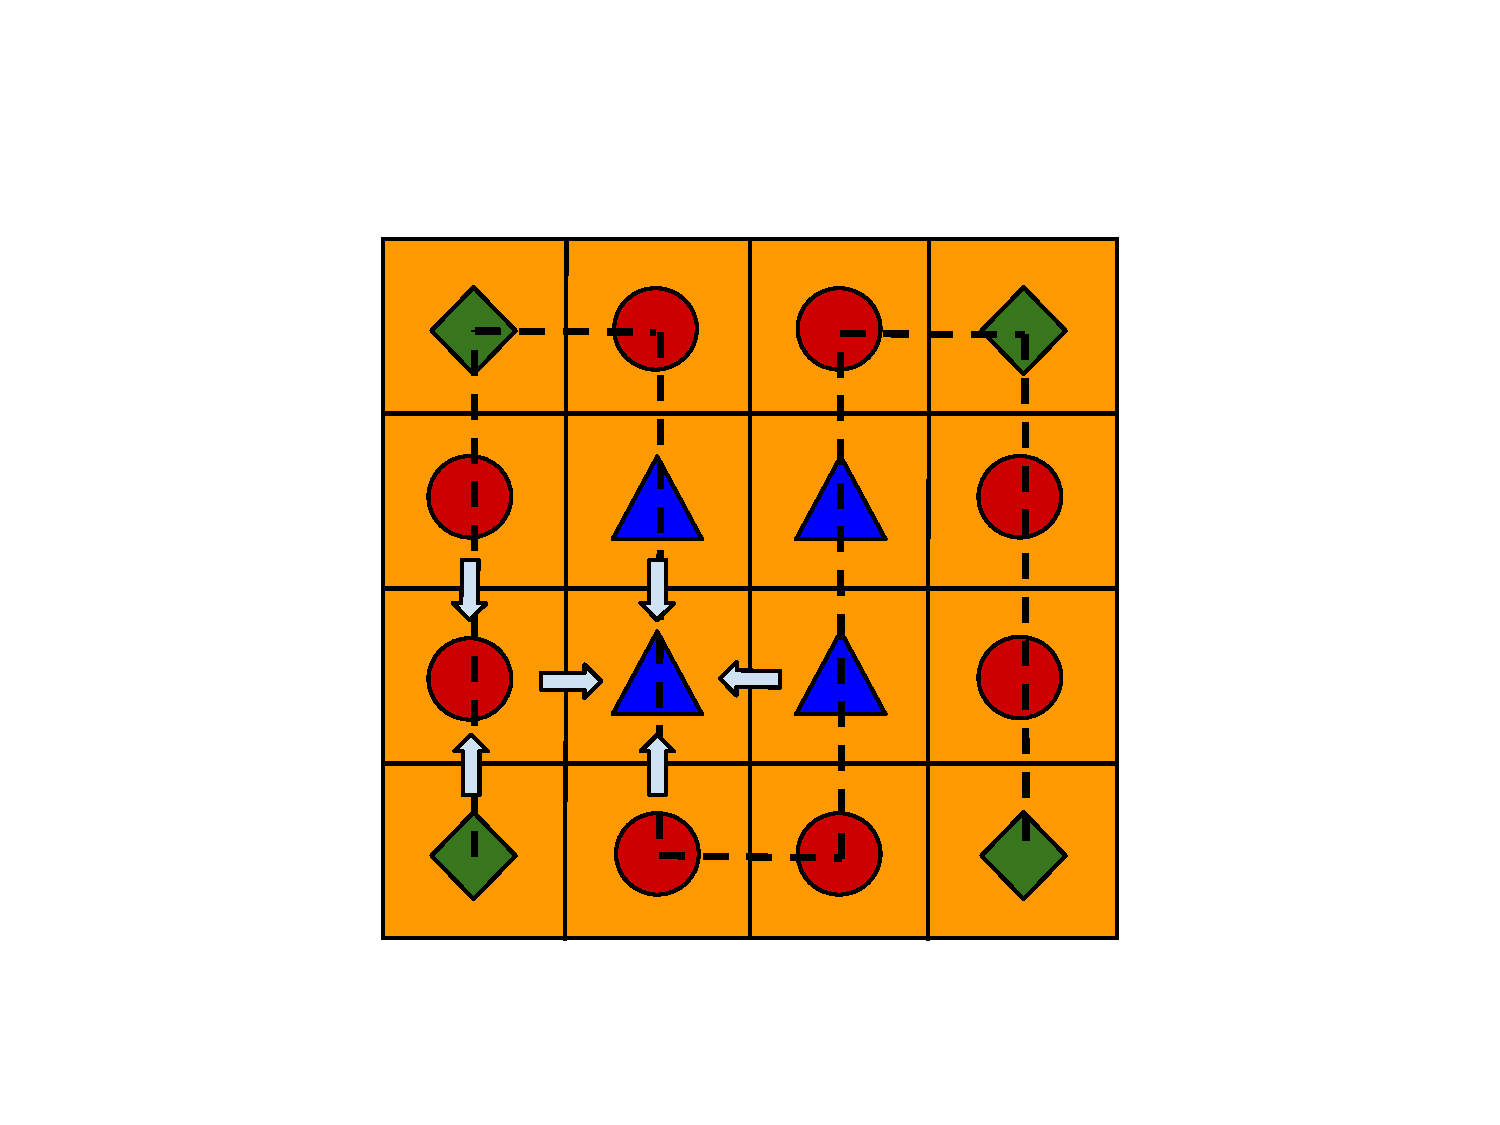
\includegraphics[scale=.35]{img/celltype.pdf}
\caption{We use different shapes to represent different cell types. We can see that it is not possible to step into a triangle cell in the memoryless deterministic reflex agent case, because an agent cannot take 2 different actions in circle cells, but which is necessary to get into the center.}
\label{fig:celltypes}
\end{figure}

\begin{verbatim}
if DIRT then SUCK 
if not DIRT and not WALL and HOME then FORWARD
if not DIRT and WALL and not HOME then RIGHT
if not DIRT and WALL and HOME then TURN OFF
if not DIRT and not WALL and not HOME then FORWARD
\end{verbatim}

So, the agent will go around the map along the boundary and return to home at the end.
